\section{Estimating the energy on a fixed fibre}\label{sec:fiber}

On a fibre at fixed $(T,\tau)$ the only positive contribution to the energy balance comes from the
wave current crossing the spatial wall $r=0$. The Gaussian is small where the current reaches the
wall, and comparison with a spatial average of the wave bounds the other factor, the boundary
value of $u/r$. This bounds the flux by a norm of the wave. To bound it by the energy itself we
recover the same norm from the interior: there we invert the Gaussian and compare $u$ with a
quadratic on each ball of radius $h$.

\begin{proposition}[\cite{OAI26}]\label{prop:fibre}
Fix $0<c_0<C_0$. There are constants $\gamma>0$, $K\ge1$ and $c,C>0$, depending only on $n$, $c_0$
and $C_0$, with the following property. Let $a=Kh$ with $0<h<1/(4K)$, and let $f$ be a
trigonometric polynomial on $\T^n=\R^n/(100\Z)^n$ with $\|f\|_2=1$ and frequencies in
$c_0/h\le|\xi|\le C_0/h$ and in the cap $|v|\le\gamma$ of some orthonormal frame. Write
$g_T=e^{-iT|D|}f$ and let $\F(T,\tau)$ be its energy from Section \ref{sec:energy}. Then
\begin{align}
\F(0,\tau)&\le Ca^2\|f\|_{\pc}^{\pc}&&(|\tau|=4a),\label{eq:Fupper}\\
\F(T,\tau)&\ge ca^2\|g_T\|_{\pc}^{\pc}&&(|\tau|=2a),\label{eq:Flower}\\
\Delta_z\F(T,\tau)&\le V(s)\,\F(T,\tau),\quad V(s)=Cs^{-2}e^{-cs/h}&&(2a\le s=|\tau|\le3).\label{eq:Fsuper}
\end{align}
The last two inequalities hold for all $T\in\R$.
\end{proposition}

\begin{proof}
Write $d=n-1$, $q=n/d=\pc/2$ and $\sigma=s/h$; throughout, $2a\le s\le3$. On the fibre
\eqref{eq:fibre} we use two regions. On $r=0$ the cut-off $g(Q)$ in the current vanishes unless
$|Q|\le1/20$, and then $|W|^2/w_0^2=1-100|Q|^2\ge3/4$, so $|W|\ge(\sqrt3/2)w_0$. Near the centre,
where $|W|\le\gamma$ and $|Q|\le1/400$, the Gaussian multiplier can be inverted. Figure
\ref{fig:fibre} shows the separation between the two regions, which lets us compare two
exponentials with different constants in their exponents. For now take $0<\gamma<w_0/8$; we
estimate uniformly in $s$, and allow the prefactor in the interior lower bound to depend on
$\gamma$.

\begin{figure}[t]
\centering
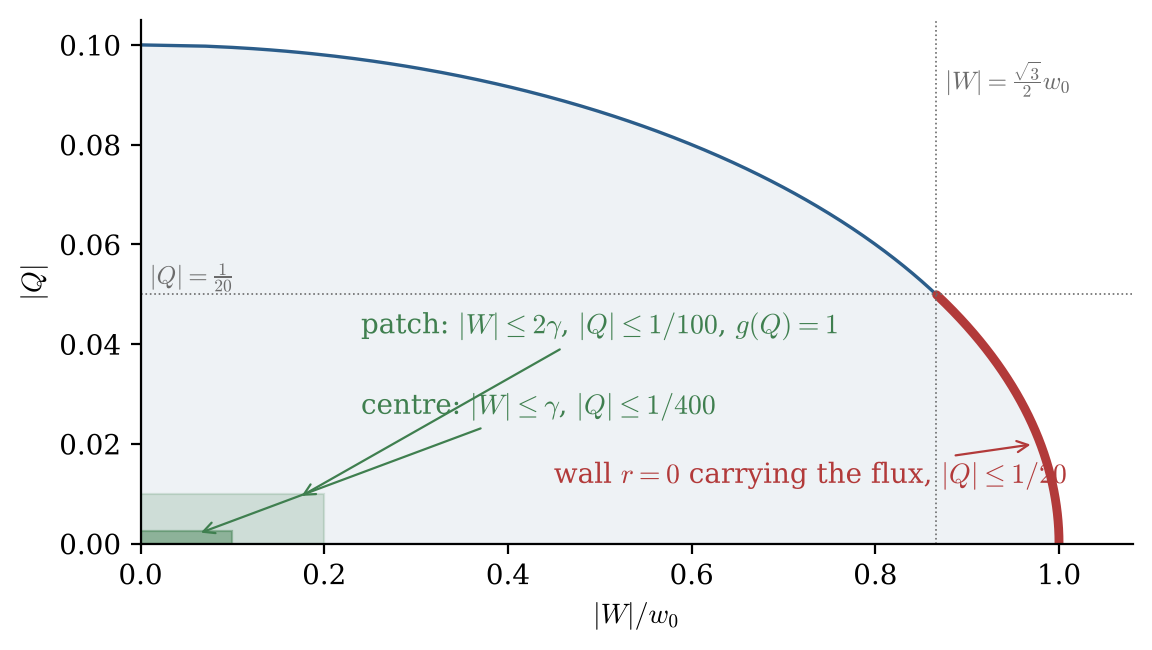
\includegraphics[width=0.92\textwidth]{figures/fig_fibre.png}
\caption{The fixed fibre in the modulus coordinates $(|W|,|Q|)$. The wave flux through the wall
$r=0$ is carried by the heavy arc, where $|Q|\le1/20$ and hence $|W|\ge\sqrt3\,w_0/2$; this
separation from the frequency cap gives the Gaussian decay $e^{-c\,s/h}$. Near the centre, balls
of radius $h$ about points with $|W|\le\gamma$, $|Q|\le1/400$ stay in the patch $|W|\le2\gamma$,
$|Q|\le1/100$, where $g(Q)=1$ and the Gaussian can be inverted at the cost $e^{C\gamma^2s/h}$.}
\label{fig:fibre}
\end{figure}

\subsubsection*{A spatial average for the upper bound}
For a dimensional constant $D\ge1$, fixed below, set
\[
P_*(X)=\bigl(J_{Ds}*|g_T|^2\bigr)(X)^{1/d},\qquad M=2n+4 ,
\]
where convolution is in the real spatial variables and $J_\ell$ is the periodisation of
$c_n\ell^{-n}(1+|X/\ell|^2)^{-M/2}$, of integral one, as in \eqref{eq:regular}. Each derivative of
this kernel costs at most a factor $C\ell^{-1}$ pointwise, $|\nabla^jJ_\ell|\le C\ell^{-j}J_\ell$; hence
$|\nabla^j(J_{Ds}*|g_T|^2)|\le C(Ds)^{-j}J_{Ds}*|g_T|^2$, and taking the $d$th root gives the first
half of
\begin{equation}\label{eq:Pstar}
|\nabla_X^jP_*|\le C(Ds)^{-j}P_*\quad(j=1,2),\qquad\int P_*^{d+1}\,dX\le\|g_T\|_{\pc}^{\pc}.
\end{equation}
The second half is Young's inequality with exponent $q=(d+1)/d$:
$\int P_*^{d+1}=\|J_{Ds}*|g_T|^2\|_q^q\le\||g_T|^2\|_q^q=\|g_T\|_{2q}^{2q}$. The positive kernel gives
$P_*>0$, since $\|g_T\|_2=1$.

We next bound the current $A_{\rm w}$ and its density $\mu$. By Proposition \ref{prop:current},
each real component of $\chi$ is the real or imaginary part of a Fourier multiplier applied to
$g_T$, whose symbol is a bounded smooth factor times
\[
(\kappa/y)^{d/2}e^{-\Psi},\qquad\Psi=\tfrac12\kappa y|W-v|^2,\qquad y=|Y|\asymp s .
\]
Multiply the symbol by a fixed smooth annular cut-off equal to one on the data and supported in
$|v|<w_0/3$. In the variable $\eta=h\xi$ its derivatives through order $M$ are bounded by
$C(hs)^{-d/2}\sigma^m$ for some fixed $m$: on this cut-off $h\kappa$ and $v$ have bounded
derivatives, $h\kappa$ is bounded away from zero, $(\kappa/y)^{d/2}\asymp(hs)^{-d/2}$, and each
derivative of $\Psi=\frac12(h\kappa)(y/h)|W-v|^2$ costs at most $C\sigma$. On the part of the wall
where $g(Q)\ne0$ we have $|W-v|\ge(\sqrt3/2-1/3)w_0$, so the same bound holds with an extra factor
$e^{-c_*\sigma}$, where $c_*>0$ does not depend on $\gamma$.

If $\mathsf B$ bounds the derivatives through order $M$ of a symbol $a(h\xi)$ supported in a fixed
compact set, then applying $(1-\Delta_\eta)^{n+2}$ inside the inverse Fourier transform bounds the
absolute value of its kernel by $C\mathsf Bh^{-n}(1+|X/h|^2)^{-M/2}$. On the torus the kernel of the
multiplier is the periodisation of the Euclidean kernel, so it is majorised by $C\mathsf BJ_h$, also
for a rotated frame. By Cauchy--Schwarz the squared modulus of the output is at most
$C\mathsf B^2J_h*|g_T|^2$. There is one more convolution with $J_h$ in $A_{\rm w}$, and
$J_h*J_h\le CJ_h$: in the Euclidean convolution one of $|Y|$, $|X-Y|$ is at least $|X|/2$, and the
inequality survives periodisation. Moreover $J_h\le(Ds/h)^nJ_{Ds}$, since
$h^{-n}(1+|X/h|^2)^{-M/2}\le(L/h)^nL^{-n}(1+|X/L|^2)^{-M/2}$ for $L=Ds\ge h$. Using
$(hs)^{-d}=s^{-2d}\sigma^d$ and enlarging $m$, we obtain, for the matrix operator norm,
\begin{equation}\label{eq:Aw}
\|A_{\rm w}\|\le Cs^{-2d}\sigma^mP_*^d\quad(r\le0),\qquad
\|A_{\rm w}\|\le Cs^{-2d}\sigma^me^{-c_*\sigma}P_*^d\quad(r=0).
\end{equation}
Only the first bound is needed for $\mu$, whose remaining term is
$h^{50n}\det\Hfib(r)\le Ch^{50n}a^{-2}s^{-2d}$ by Lemma \ref{lem:fibre}. The nearest lattice term of
the kernel gives $\inf_XJ_{Ds}(X)\ge c_Dh^{M-n}$, since the torus has fixed diameter and $h\le s\le3$;
consequently $P_*^d\ge c_Dh^{M-n}\|g_T\|_2^2=c_Dh^{M-n}$, which absorbs $h^{50n}a^{-2}\le h^{50n-2}$.
In particular
\begin{equation}\label{eq:mu}
\mu\le Cs^{-2d}\sigma^mP_*^d\qquad(r\le0).
\end{equation}

\subsubsection*{A comparison function vanishing on the wall}
Put $R=\Hfib(r)$. By Lemma \ref{lem:fibre}, $R\ge cs^{-2}I$ and $\Gfib(r)\Gfib(r)^*\le R$. We claim
\begin{equation}\label{eq:rPstar}
\Hfib(rP_*)\ge(1-C/D)P_*R .
\end{equation}
The product rule \eqref{eq:product} gives $P_*R$, $r\Hfib(P_*)$ and two terms pairing the
gradients of $r$ and $P_*$. For a quaternionic vector $e$, $|e^*\Gfib(r)|\le(e^*Re)^{1/2}$, while
$|e^*\Gfib(P_*)|\le|\nabla P_*||e|\le C(Ds)^{-1}P_*\cdot Cs(e^*Re)^{1/2}$ by \eqref{eq:Pstar} and
$R\ge cs^{-2}I$; this bounds the mixed terms by $CD^{-1}P_*e^*Re$. The term with $\Hfib(P_*)$ is at
most $C(Ds)^{-2}P_*|e|^2\le CD^{-2}P_*e^*Re$ by \eqref{eq:Pstar} and $|r|\le1$.

Since $r<0$, an upper bound for $u/r$ calls for a comparison function below $u$ whose
determinant is at least $\lambda\mu$. Fix $D$ so that the right side of \eqref{eq:rPstar} is at
least $P_*R/2$. For $v_*=C_1\sigma^{m_1}rP_*$ this gives $\Hfib(v_*)\ge\alpha I$ with
$\alpha=cC_1\sigma^{m_1}P_*s^{-2}$. The background $B_{\rm fib}=\lambda\Hfib(|\Phi|^2)$ has rank one
and positive eigenvalue $\beta\asymp\lambda$ by Lemma \ref{lem:fibre}, so by the monotonicity of
$\det$ in Lemma \ref{lem:moore} and \eqref{eq:compress},
\[
\det\bigl(B_{\rm fib}+\Hfib(v_*)\bigr)\ge\det(B_{\rm fib}+\alpha I)=(\beta+\alpha)\alpha^d
\ge c\lambda\bigl(C_1\sigma^{m_1}P_*s^{-2}\bigr)^d\ge\lambda\mu ,
\]
by \eqref{eq:mu}, once $m_1d\ge m$ and $C_1$ is large. The potentials $v_*$ and $u$ have the same
zero boundary values, so the comparison principle in the proof of Theorem \ref{thm:dirichlet}
yields $v_*\le u\le0$. Dividing by $r<0$ and passing to the boundary,
\begin{equation}\label{eq:urho}
0\le u/r\le C_1\sigma^{m_1}P_*\qquad(r\le0).
\end{equation}

By Lemma \ref{lem:comparison}, $\F\le X_0=\int(-u)\mu\,d\zeta$, and $-u=|r|\,(u/r)\le C_1\sigma^{m_1}P_*$.
The volume element in $(P,Z)$ is comparable to $a^2s^{2d}\,dW\,dQ$ on a fixed bounded set, by Lemma
\ref{lem:fibre}, and $P_*$ depends only on $X$. Combining \eqref{eq:Pstar}, \eqref{eq:mu} and
\eqref{eq:urho} therefore gives, after enlarging $m$,
\begin{equation}\label{eq:Fup}
\F(T,\tau)\le Ca^2\sigma^m\|g_T\|_{\pc}^{\pc}.
\end{equation}
For the flux we need the full gradient of $r$. Tangency in Proposition \ref{prop:current} gives
$A_{\rm w}G(|\Phi|^2)=0$, because $G(|\Phi|^2)=2(\partial\Phi)^*\Phi\,\ii$; the remaining part
$w_0^{-2}G(|W|^2)$ has size $O(s^{-1})$ by Lemma \ref{lem:fibre}. Thus
$G(r)^*A_{\rm w}G(r)\le Cs^{-2}\|A_{\rm w}\|$. In the coordinates $(W,Q)$ the function $r$ is fixed
with nonvanishing gradient on the wall, so the coarea formula and Lemma \ref{lem:fibre} give
$\int\delta(r)\,dP\,dZ\le Ca^2s^{2d}$. Inserting the wall bound \eqref{eq:Aw} and \eqref{eq:urho}
into the flux integral of Proposition \ref{prop:balance},
\begin{equation}\label{eq:fluxbound}
\Delta_z\F(T,\tau)\le C(a/s)^2\sigma^me^{-c_*\sigma}\|g_T\|_{\pc}^{\pc}.
\end{equation}

\subsubsection*{Recovering the wave in the interior}
Consider a centre $(X,P,Z)$ with $|W|\le\gamma$ and $|Q|\le1/400$. In the ball of radius $h$
about it in the $3n$ real spatial coordinates, $W=P/Y$ changes by at most $Ch/s\le C/K$ and
$\Phi$ by at most $Ch$, so $Q$ by at most $C/K$. If $K\gamma$ and $K$ are large enough, the ball
lies in $|W|\le2\gamma$, $|Q|\le1/100$, inside the fibre, and the cut-off in $A_{\rm w}$ equals one
throughout it.

The first scalar multiplier $S_0$ of the time component in \eqref{eq:ATT} has symbol
$b_0(\kappa/y)^{d/2}e^{-\Psi}$ with $b_0=(1+\Re(W)\cdot v/2)/\sqrt2$ bounded away from zero, and the
other component is orthogonal, so $|S_0g_T|^2\le A^0_{TT}$. Invert $S_0$ on the frequencies of
$g_T$ by multiplying its reciprocal symbol by a smooth annular cut-off equal to one on the data
and supported in $|v|\le2\gamma$. On its support $|W-v|\le4\gamma$, so $\Psi\le C\gamma^2\sigma$, and
the derivatives of the reciprocal symbol in $\eta=h\xi$ through order $M$ are bounded by
\[
\mathsf B_{\rm inv}=C_\gamma(hs)^{d/2}\sigma^me^{C\gamma^2\sigma};
\]
the derivatives of the cut-off enter only the prefactor $C_\gamma$, and the constant in the
exponential does not depend on $\gamma$. The kernel estimate above yields
$|g_T(X)|^2\le C\mathsf B_{\rm inv}^2(J_h*A^0_{TT})(X)$ for each choice of the imaginary coordinates
in the ball, with $A^0_{TT}$ evaluated at those coordinates. Since $J_h(X-Y)$ and $J_h(X'-Y)$ are
comparable for $|X'-X|\le h$, the density at every point of the ball is at least
\begin{equation}\label{eq:mX}
m_X=c_\gamma(hs)^{-d}\sigma^{-m}e^{-C_2\gamma^2\sigma}|g_T(X)|^2 .
\end{equation}

For the interior lower bound on $-u$ we need a comparison function above $u$. Let $l$ be the
Euclidean distance from the centre. The quadratic $v_b=\eps m_X^{1/d}(l^2-h^2)$ vanishes on the
boundary of the ball and has fibre Hessian $6\eps m_X^{1/d}I$, since there are three real slots
per spatial coordinate. If $m_X>0$, its determinant after adding $B_{\rm fib}$ is
\[
(\beta+6\eps m_X^{1/d})(6\eps m_X^{1/d})^d\le C\bigl((\eps m_X^{1/d})^n+\lambda(\eps m_X^{1/d})^d\bigr)
\le C(\eps^n+\eps^d)\lambda m_X\le\lambda m_X ,
\]
for a fixed small $\eps$, because the density ceiling \eqref{eq:lambda} and \eqref{eq:mX} give
$m_X^{1/d}\le\mu^{1/d}\le\lambda$. Now $u\le0=v_b$ on the boundary of the ball and the
determinant of $B_{\rm fib}+\Hfib(u)$ is $\lambda\mu\ge\lambda m_X$, so the comparison principle on
the ball (Theorem \ref{thm:dirichlet} and its proof) gives $u\le v_b$ there. At the centre the
depth is therefore at least $\eps h^2m_X^{1/d}$, and multiplying by $\mu\ge m_X$ gives
$(-u)\mu\ge\eps h^2m_X^{1+1/d}$, also when $m_X=0$. Here $1+1/d=q$, and $m_X^q$ contains
$|g_T(X)|^{2q}=|g_T(X)|^{\pc}$.

The imaginary volume of the region of centres is comparable to $a^2s^{2d}\gamma^{2d}$. Integrate
the centre inequality over it and over $X$, use the lower bound of Lemma \ref{lem:comparison}, and
note that $h^2s^{2d}(hs)^{-dq}=h^{1-d}s^{d-1}=\sigma^{n-2}$ since $dq=d+1$. Enlarging $m$ and
absorbing $\gamma^{2d}$ into the prefactor,
\begin{equation}\label{eq:Flow}
\F(T,\tau)\ge c_\gamma a^2\sigma^{-m}e^{-C_3\gamma^2\sigma}\|g_T\|_{\pc}^{\pc}.
\end{equation}

Choose $\gamma$ so small that $C_3\gamma^2<c_*/2$, then fix $K$ to meet the ball inclusions and so
that $h<1/(4K)$ lies in the range of \eqref{eq:lambda}. For $f\ne0$ both sides below are positive,
and dividing \eqref{eq:fluxbound} by \eqref{eq:Flow} gives
\[
\frac{\Delta_z\F}{\F}\le C_\gamma s^{-2}\sigma^{2m}e^{-(c_*-C_3\gamma^2)\sigma}.
\]
The exponential absorbs the power of $\sigma$, which proves \eqref{eq:Fsuper}. On the two circles
in the $\tau$-plane the scaled radii $4a/h=4K$ and $2a/h=2K$ are fixed. The upper bound
\eqref{eq:Fup} at $T=0$ on the first circle gives \eqref{eq:Fupper}, and the lower bound
\eqref{eq:Flow} on the second gives \eqref{eq:Flower} for the wave at time $T$.
\end{proof}
